\section{Power consumption estimation}
In this section, there is a description of the power consumption of the ESP32 node in all states: deep sleep, idle, sensor reading, WiFi turned on and transmission.\\
In order to estimate power consumption based on the provided CSV files, we first plotted data using Python and Matplotlib library. Based on the plot, we computed the average power consumption in the analyzed working state.

\subsection{Power consumption plots}
In order to plot the data contained in the provided CSV files, we used the following algorithm.

\begin{python}
import pandas as pd
import matplotlib.pyplot as plt
# read CSV file 
df = pd.read_csv('deep_sleep.csv', parse_dates=['Timestamp'])
# plot data
plt.figure(figsize=(10, 6))
plt.plot(df['Timestamp'], df['Data'], linestyle='-', linewidth=2)
plt.xlabel('Time')
plt.ylabel('Power [mW]')
plt.title('Power consumption deep sleep')
plt.grid(True)
# save and shows
plt.savefig("power_consumption_deep_sleep.pdf", format="pdf", bbox_inches="tight")
plt.show()
\end{python}

\subsubsection{Power consumption deep\_sleep.csv}
The following plot represents the power consumption when the ESP32 is in deep sleep state (lowest power level), goes into idle mode (medium power level) and finally turns the WiFi on (highest power level). 
\begin{figure}[H]
    \centering
    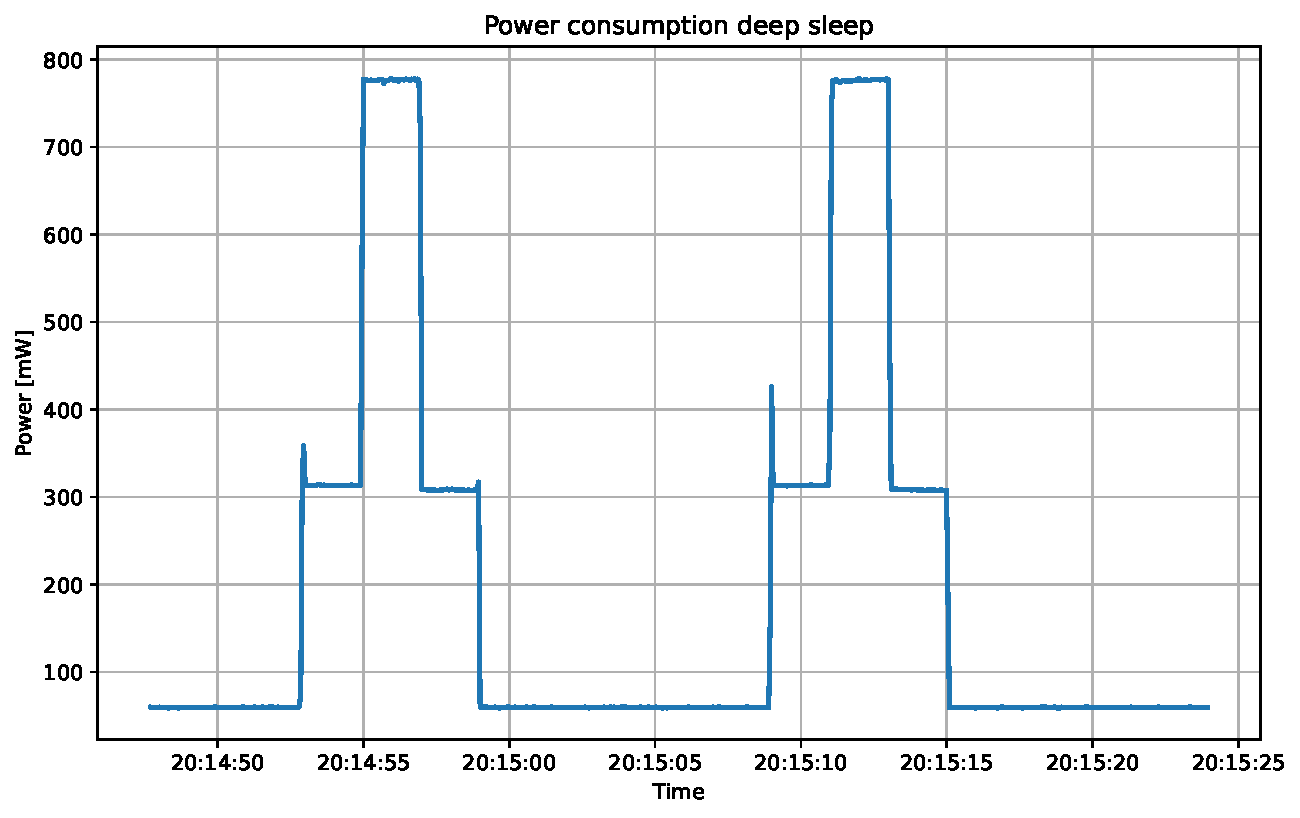
\includegraphics[width=\linewidth, height=0.4\textheight, keepaspectratio]{power_consumption_deep_sleep.pdf}
    \caption{Power consumption deep sleep state}
    \label{fig:Power consumption deep sleep state}
\end{figure}

\subsubsection{Power consumption sensor\_read.csv}
The following plot represents the power consumption when the ESP32 alternates the idle mode and sensor reading mode, in which it performs a measurement using the ultrasonic distance sensor HC-SR04.
\begin{figure}[H]
    \centering
    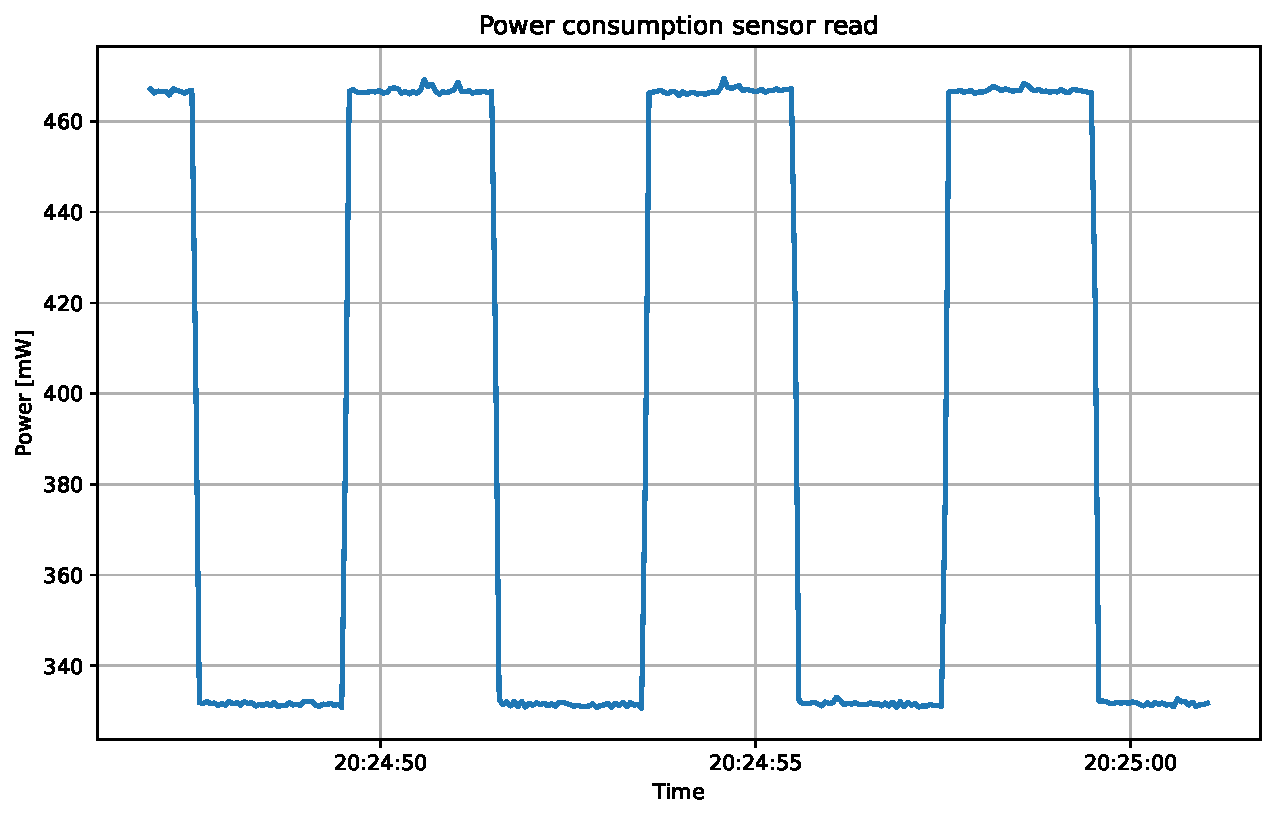
\includegraphics[width=\linewidth, height=0.4\textheight, keepaspectratio]{power_consumption_sensor_read.pdf}
    \caption{Power consumption deep sleep state}
    \label{fig:Power consumption deep sleep state}
\end{figure}

\subsubsection{Power consumption transmission\_power.csv}
The following plot represents the power consumption when the ESP32 has the WiFi turned on and transmits data using ESP-NOW at 19.5 dBm and 2 dBm.
\begin{figure}[H]
    \centering
    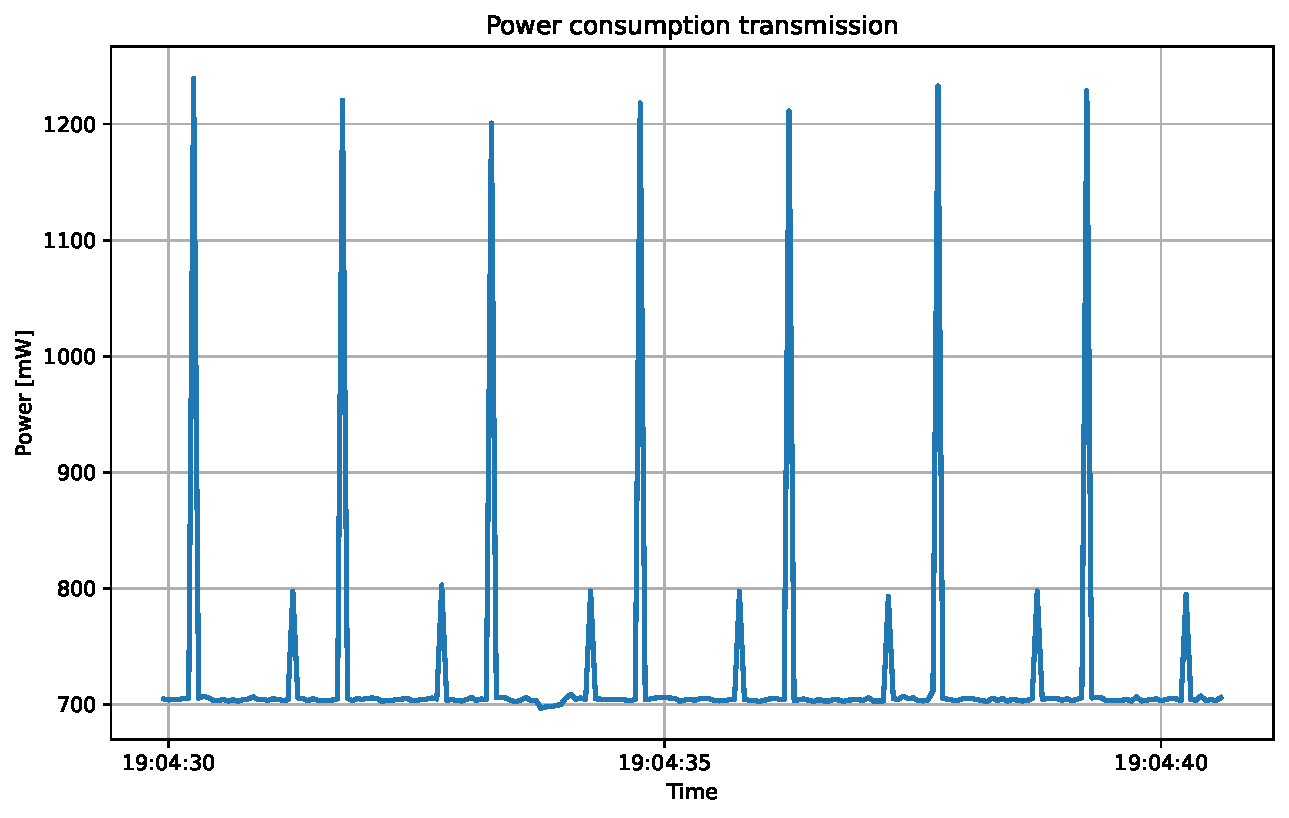
\includegraphics[width=\linewidth, height=0.4\textheight, keepaspectratio]{power_consumption_transmission.pdf}
    \caption{Power consumption deep sleep state}
    \label{fig:Power consumption deep sleep state}
\end{figure}

\subsection{Average power consumption values}
In order to find a numerical estimation of the power consumption in different states, we used some Python algorithms, using the library Pandas. Starting from the plot we selected the range of values regarding a particular state, discarding the others, and computed the average power consumption. For some states, the values of power can be found in multiple CSV files; in such cases, we merged different files in order to have a more accurate estimation.\\
In the following sections we also report two example of algorithms used to compute the average, both using a single dataset and multiple datasets.

\subsubsection{Power consumption in deep sleep state}
Data to estimate the deep sleep mode is contained in the dataset deep\_sleep.csv. We filtered all values of power above 100mW, referring to other states as shown by the plot, and computed the average.

\begin{python}
import pandas as pd 
# read CSV file 
dataset_deep_sleep = pd.read_csv("deep_sleep.csv", parse_dates=['Timestamp'])
# filter data with power < 100mW, referring to deep sleep mode
deep_sleep_data = dataset_deep_sleep[dataset_deep_sleep["Data"] < 100]
# compute average
deep_sleep_avg_power = deep_sleep_data["Data"].mean()
# print average 
print("Average power consumption deep sleep: ", deep_sleep_avg_power)
\end{python}

We obtained an average consumption in deep sleep of 59.66 mW.

\subsubsection{Power consumption in idle state}
The power consumption in idle state can be extracted both by sensor\_read.csv and transmission\_power.csv. We used both datasets, merging all values and computing the average. We considered only values between 200 mW and 500 mW, that refer to idle mode.
\begin{python}
import pandas as pd 
# read CSV file 
dataset_deep_sleep = pd.read_csv("deep_sleep.csv", parse_dates=['Timestamp'])
dataset_sensor_reading = pd.read_csv("sensor_read.csv", parse_dates=['Timestamp'])
# filter data with power between 200 mW and 500 mW, referring to idle mode
idle_data_deep_sleep = dataset_deep_sleep[(dataset_deep_sleep['Data'] >= 200) & (dataset_deep_sleep['Data'] <= 500)]
# filter data with power <= 400 mW, reffering to idle mode
idle_data_sensor_reading = dataset_sensor_reading[dataset_sensor_reading['Data'] <= 400]
# merge values 
idle_merged = pd.concat([idle_data_deep_sleep, idle_data_sensor_reading], ignore_index=True)
# compute average
idle_avg_power = idle_merged['Data'].mean()
# print average 
print("Average power consumption idle: ", idle_avg_power)
\end{python}

We obtained an average consumption in idle of 322.62 mW.

\subsubsection{Power consumption in measurement state}
Data representing power consumption in measurement state is contained in the dataset sensor\_read.csv. We computed the average value considering values of power above 400 mW and obtained an average value of 465.18 mW. The algorithm is very similar to deep sleep mode, thus we don't report it.

\subsubsection{Power consumption in WiFi on state}
We estimated the power consumption when the WiFi is turned on and the ESP32 is not transmitting based on deep\_sleep.csv and transmission\_power.csv, merging all value between 600 mW and 750 mW, as shown for the idle mode. The average power consumption when WiFi is turned on is 724.58 mW.

\subsubsection{Power consumption when transmitting at 2 dBm}
Finally, we estimated the average power consumption when ESP32 is transmitting at 2 dBm, based on transmission\_power.csv. We compute the average of values between 750 mW and 900 mW, obtaining an average value of 797.29 mW.

\subsubsection{Summary power consumption}
The summary of power consumption of ESP32 in different states is reported below.

\begin{table}[H]
\centering 
\begin{tabular}{| c | c |}
	\hline 
	\rowcolor{bluepoli!40}
	\textbf{State} & \textbf{Power}\T\B \\
	\hline 
	$P_{idle}$ & $322.62\,\text{mW}$ \T\B\\
	$P_{measurement}$ & $465.18\,\text{mW}$ \T\B\\
	$P_{WiFi}$ & $724.58\,\text{mW}$ \T\B\\
	$P_{transmission}$ & $797.29\,\text{mW}$ \T\B\\
	$P_{deep\_sleep}$  & $59.66\,\text{mW}$ \T\B\\
	\hline
\end{tabular}
\\[10pt]
\caption{States power table}
\label{table:states_power_table}
\end{table}

\section{States duration estimation}
We estimated the duration of different states by simulating the ESP32 on Wokwi and measuring them. We saved the timestamps in different points of execution, computed the duration of each state and printed it on the serial log.\\
We simulated the execution for about a hundred cycles and saved the serial log. We provide few examples of entries of the serial log, in which the durations are in microseconds.

\begin{verbatim}
entry 0x400805dc
Idle duration: 882
Measurement duration: 24116
Sending duration: 64
WiFi duration: 189158
ets Jul 29 2019 12:21:46

entry 0x400805dc
Idle duration: 846
Measurement duration: 24212
Sending duration: 65
WiFi duration: 188548
ets Jul 29 2019 12:21:46

entry 0x400805dc
Idle duration: 845
Measurement duration: 24211
Sending duration: 64
WiFi duration: 187548
ets Jul 29 2019 12:21:46
\end{verbatim}

We computed the duration of different states using a Python algorithm to extract the values from the log, using regexes, filtering outliers and computing the average. \\
In the measurement of the sending duration, during which the ESP32 uses WiFi, we noticed the presence of some values completely different from the others, caused by the simulation on Wokwi; we filtered them out to get a more accurate estimation. \\
Finally, we observed that the duration of the measurement with the HC-SR04 ultrasonic distance sensor varies based on the resulting distance: the higher the distance, the longer the duration. In order to have a realistic duration, we gathered data with different values of measured distance.

\begin{python}
import re
import statistics
# open log file
with open("time_measurements_log.txt", "r") as file:
    log_text = file.read()
# extract values from log using a regex 
idle_values = list(map(int, re.findall(r"Idle duration:\s*(\d+)", log_text)))
measurement_values = list(map(int, re.findall(r"Measurement duration:\s*(\d+)", log_text)))
sending_values = list(map(int, re.findall(r"Sending duration:\s*(\d+)", log_text)))
wifi_values = list(map(int, re.findall(r"WiFi duration:\s*(\d+)", log_text)))
# filter wrong values, given by the simulation
wifi_values = [value for value in wifi_values if value <= 200000]
# compute averages
avg_idle = statistics.mean(idle_values) if idle_values else 0
avg_measurement = statistics.mean(measurement_values) if measurement_values else 0
avg_sending = statistics.mean(sending_values) if sending_values else 0
avg_wifi = statistics.mean(wifi_values) if wifi_values else 0
#print values
print("Average Idle duration:", avg_idle)
print("Average Measurement duration:", avg_measurement)
print("Average Sending duration:", avg_sending)
print("Average WiFi duration:", avg_wifi)
\end{python}

The deep sleep duration is computed from the last two digits of the person code, 10773593, as:
\begin{align*}
	T_{deep\_sleep} &= (93 \% 50) + 5 = 48\,\text{s} \\ 
\end{align*}

The duration of different states is reported in the following table.

\begin{table}[H]
\centering 
\begin{tabular}{| c | c |}
	\hline 
	\rowcolor{bluepoli!40}
	\textbf{State} & \textbf{Duration}\T\B \\
	\hline 
	$T_{idle}$ & $833.70\,\mu\text{s}$ \T\B\\
	$T_{measurement}$ & $18647.79\,\mu\text{s}$ \T\B\\
	$T_{WiFi}$ & $188640.86\,\mu\text{s}$ \T\B\\
	$T_{transmission}$ & $59.60\,\mu\text{s}$ \T\B\\
	$T_{deep\_sleep}$  & $48\times10^6\,\mu\text{s}$ \T\B\\
	\hline
\end{tabular}
\\[10pt]
\caption{States duration table}
\label{table:states_duration_table}
\end{table}

\section{Energy consumption estimation}
Starting from the power consumption and states durations estimations, we can easily compute energy consumed by the ESP32 by multiplying the power and the time of each state.\\
At start, the ESP32 is in idle mode for T\_{idle}. Then it enters measurement mode to measure the distance with the ultrasonic distance sensor HC-SR04 for T\_{measurement}. When the measurement is completed, the ESP32 turns the WiFi on for T\_{WiFi} and, during this same period, it transmits data at 2 dBm for T\_{transmission}. Finally, it enters deep sleep for T\_{deep\_sleep}. \\

The energy for different states is computed as follows.
\begin{align*}
	E_{idle} &= P_{idle} \cdot T_{idle} = 0.268 \,\text{mJ} \\ 
	E_{measurement} &= P_{measurement} \cdot T_{measurement} = 8.675 \,\text{mJ} \\
	E_{WiFi} &= P_{WiFi} \cdot \Bigl(T_{WiFi} - T_{transmission} \Bigr) = 136.642\,\text{mJ} \\
	E_{transmission} &= P_{transmission} \cdot T_{transmission} = 0.048\,\text{mJ} \\
   	E_{deep\_sleep} &= P_{deep\_sleep} \cdot T_{deep\_sleep} = 2863,680\,\text{mJ} 
\end{align*}

The energy consumption for a cycle is computed as the sum.
\[
E_{cycle} = E_{idle} + E_{measurement} + E_{WiFi} + E_{transmission} + E_{deep\_sleep} = 3009,313\,\text{mJ} 
\]

The available energy is computed from the last four digits of the person code, 10773593, as: 
\begin{align*}
	E_{b} &= (3593 \% 5000) + 15000 = 18593\,\text{J} = 18593000\,\text{mJ}
\end{align*}

The sensor node has a lifetime, measured in cycles, of:
\begin{align*}
	L_{cycles}&= E_{b}/E_{cycle} = 6178.487 \,\text{cycles} 
\end{align*}

The total time for a cycle is:
\begin{align*}
	T_{cycle} &= T_{idle} + T_{measurement} + T_{WiFi} + T_{deep\_sleep} = 48.208 \text{s}
\end{align*}

The lifetime, measured in time, is of:
\begin{align*}
	L_{time}&= L_{cycles} \cdot T_{cycle} = 297852.501 \text{s}
\end{align*}

The lifetime is equivalent to 3 days, 10 hours, 44 minutes and 12 seconds.


